% ===================== ANÁLISIS =====================
\section{Análisis}

\subsection{Diagrama Esquemático de la Caldera}

\begin{figure}[H]
    \centering
    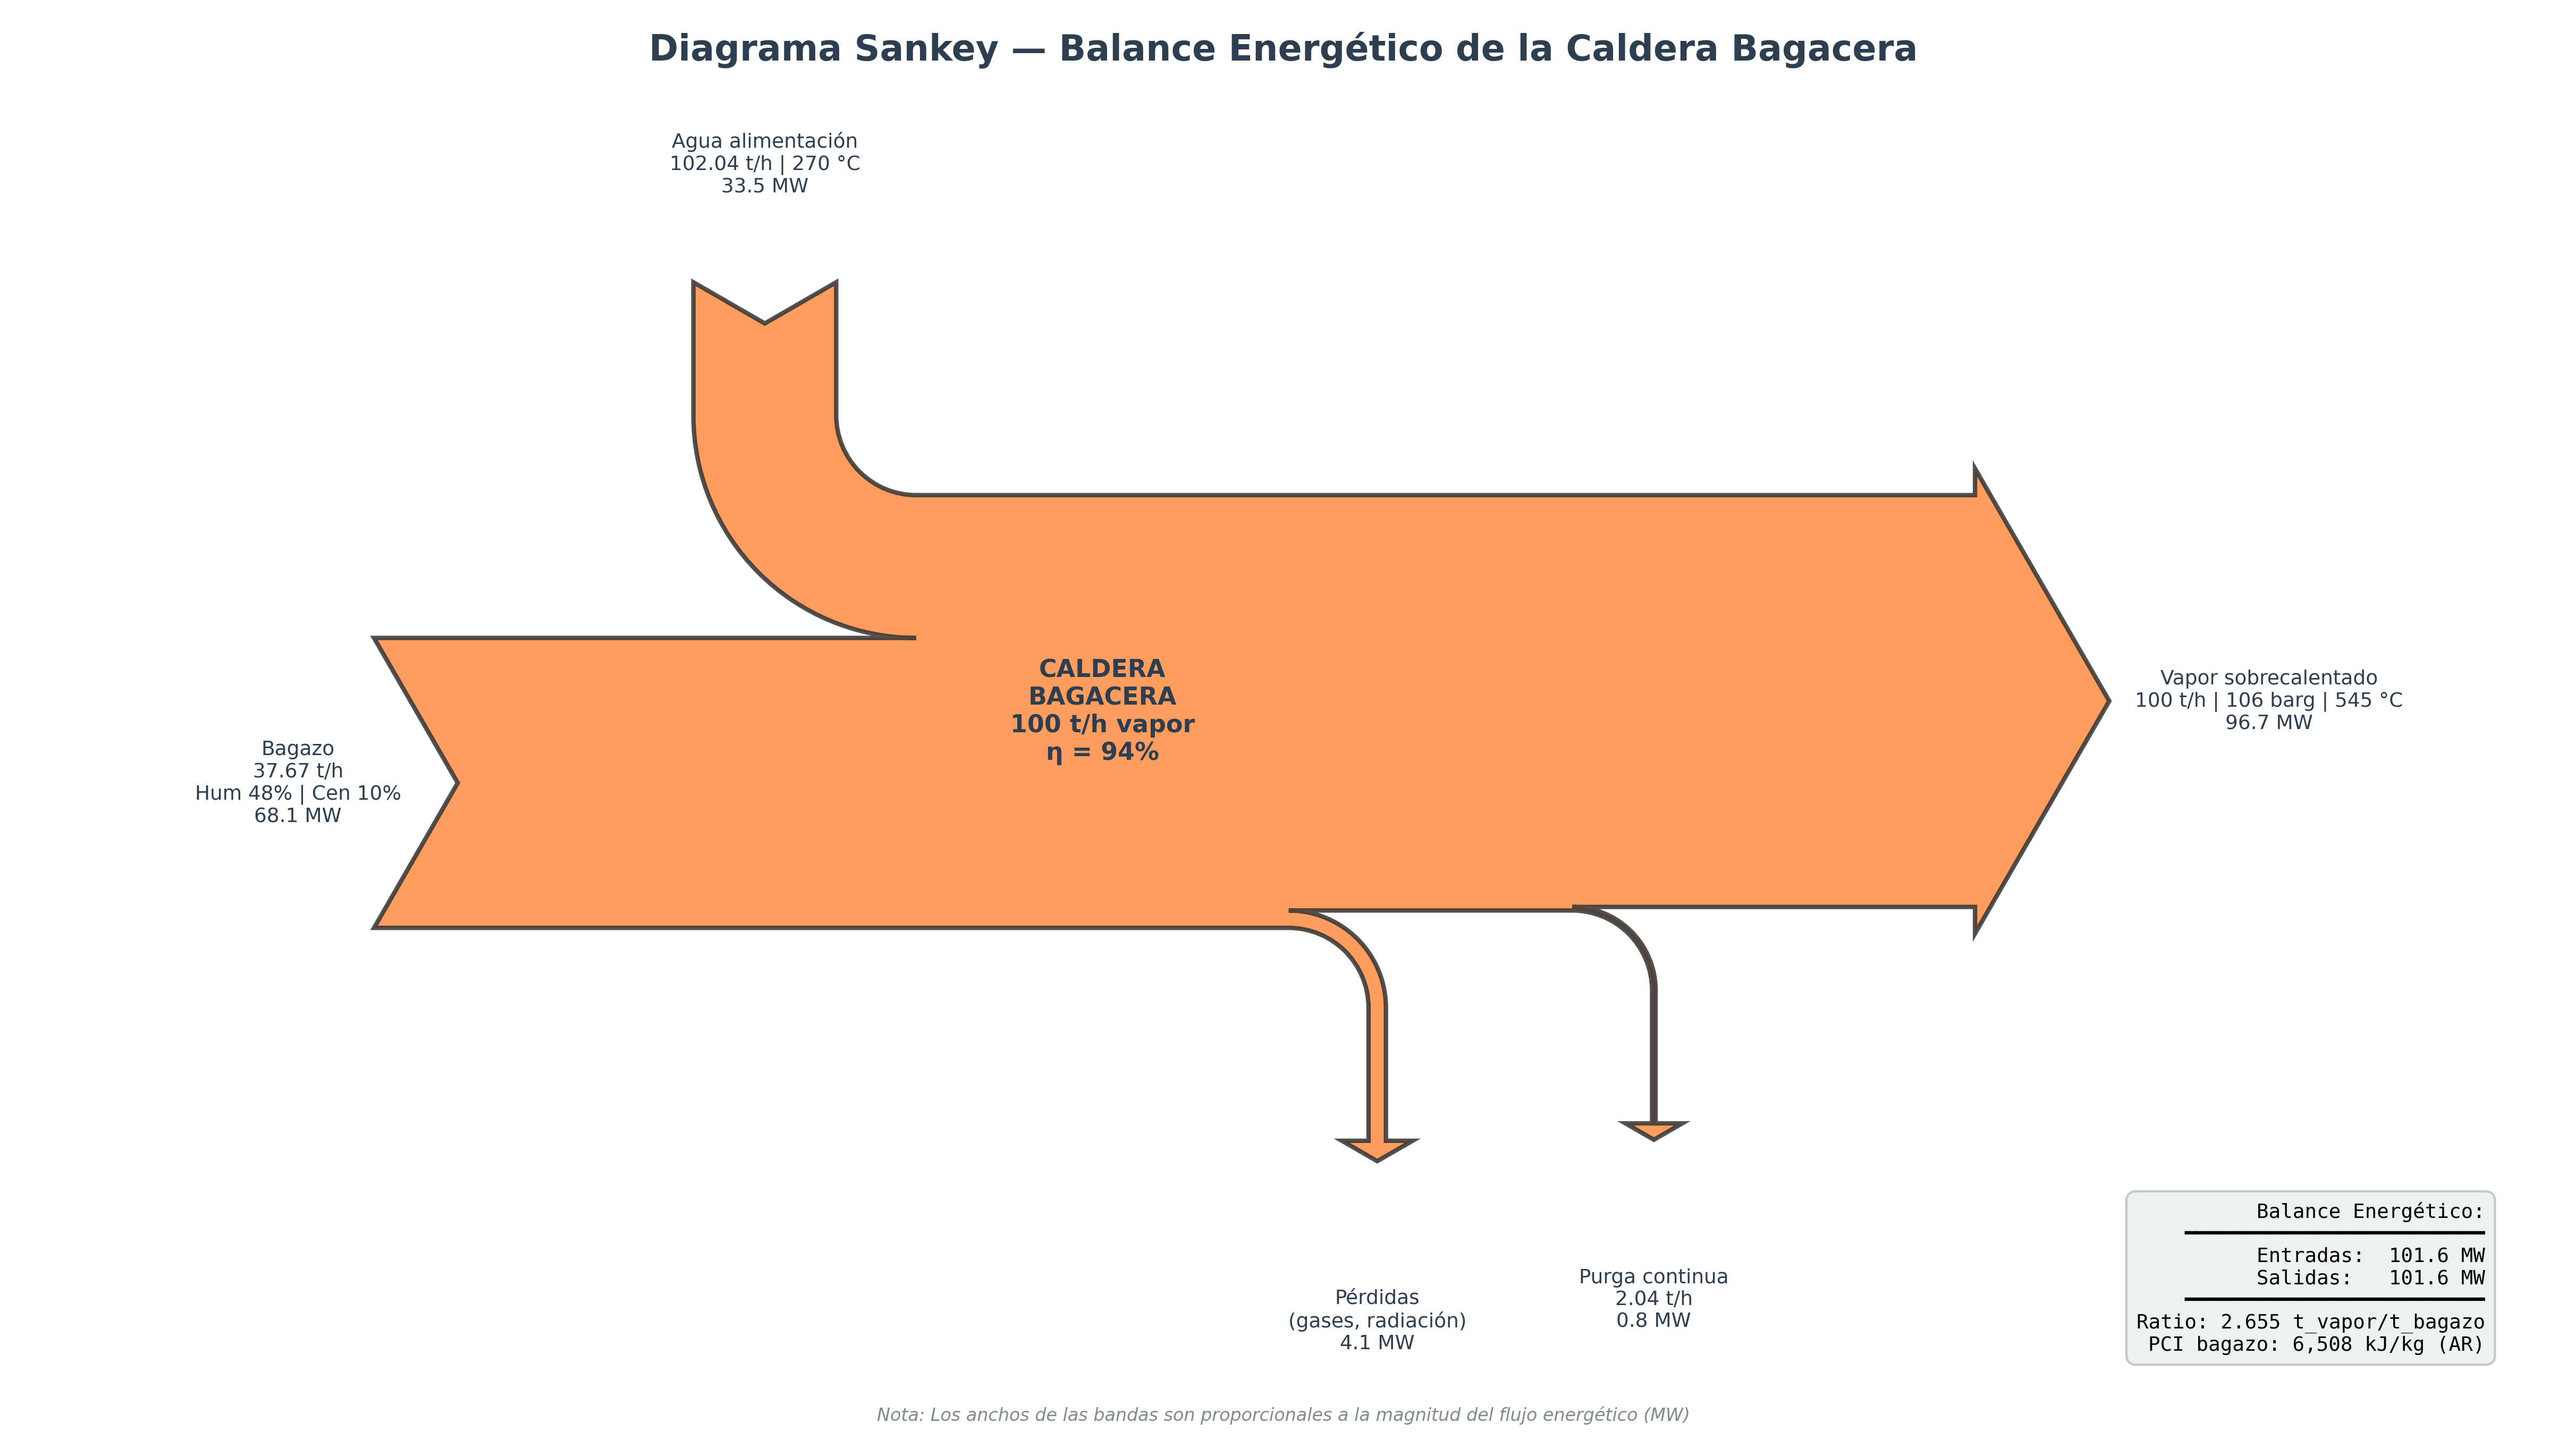
\includegraphics[width=0.95\textwidth]{assets/fig_diagrama_caldera.pdf}
    \caption{Diagrama Sankey del balance energético de la caldera bagacera}
    \label{fig:diagrama_caldera}
\end{figure}

La Figura~\ref{fig:diagrama_caldera} muestra el esquema de flujo de la caldera bagacera, identificando los equipos principales (hogar de combustión, domo separador, sobrecalentador y economizador) junto con las corrientes de entrada y salida. El calor absorbido por el fluido de trabajo ($Q_{abs} = 64$~MW) se transfiere desde el hogar hacia los haces tubulares del sobrecalentador, mientras que la circulación natural conecta el domo con el hogar a través de los tubos de agua descendentes y ascendentes.

\subsection{Discusión de Resultados}

El ratio obtenido de \textbf{2.655 t de vapor por tonelada de bagazo} refleja un escenario conservador de diseño, consistente con las condiciones de operación más exigentes de la agroindustria cañera colombiana. Los factores que justifican este resultado:

\begin{enumerate}
	\item \textbf{Humedad del 48\%:} Representa la condición estándar de operación del tándem de molinos sin secado mecánico adicional. La humedad es el factor dominante en la penalización del PCI: casi la mitad de la masa del bagazo es agua que debe evaporarse antes de que la combustión sea efectiva.
	\item \textbf{Cenizas del 10\% (AR):} Este valor incluye no solo las cenizas intrínsecas del bagazo ($\sim$2--3\% BS) sino también la materia extraña mineral que ingresa al hogar de combustión: tierra de cosecha mecanizada, arena, y partículas silíceas. Este valor constituye un factor de diseño conservador que garantiza el dimensionamiento adecuado del equipo.
	\item \textbf{Fracción combustible resultante (42\%):} Solo el 42\% de la masa del bagazo tal como se recibe es materia orgánica combustible. El restante 58\% (agua + cenizas) no contribuye energéticamente y debe ser manejado por el sistema de combustión y extracción de cenizas.
	\item \textbf{Ratio en contexto industrial:} Para calderas de alta presión ($>$60 bar) en ingenios colombianos, los ratios reportados varían entre 2.0 y 3.5 t$_{\text{vapor}}$/t$_{\text{bagazo}}$, dependiendo de la calidad del combustible y las condiciones del vapor. El valor de 2.655 se ubica en el rango bajo-medio, coherente con la combinación de alta humedad y alto contenido mineral adoptada.
\end{enumerate}
